\chapter{General Project Presentation}

\section*{Introduction}
\addcontentsline{toc}{section}{Introduction}

This chapter introduces the host organization, frames the project context, compares the BVIRAL
Platform with existing market solutions, and presents the Agile methodology, the sprint planning,
and the overall timeline followed during the project.

%% ─── 1.1 ─────────────────────────────────────────────────────────────────────
\section{Presentation of the Host Organization}

\subsection{BVIRAL Media Inc.}

\textbf{BVIRAL} is a digital media company that licenses viral video content. It acts as an
intermediary between \textit{content creators}, individuals who capture footage on Instagram,
TikTok, YouTube, and Facebook, and \textit{media buyers}, such as news outlets, broadcasters,
publishers, and advertising agencies that need licensed footage for production.

BVIRAL's business model includes:

\begin{itemize}
  \item Discovering and curating high-engagement video clips from social media.
  \item Acquiring exclusive or non-exclusive licensing rights from creators.
  \item Indexing content for fast retrieval.
  \item Sub-licensing to media partners through a SaaS subscription.
\end{itemize}

The platform developed in this project serves both sides of this marketplace through two front-end
portals backed by a shared API layer.

\subsection{Technical Environment Before This Project}

Before the unified BVIRAL Platform, the company relied on a mix of internal scripts and external
SaaS tools, each managing a separate part of the business (creator management, payments, video
archives). There was no shared data model, no self-service onboarding, and onboarding a new client
required manual work across multiple systems.

%% ─── 1.2 ─────────────────────────────────────────────────────────────────────
\section{Project Presentation}

\subsection{Objectives}

This project was commissioned to design and build a unified, production-ready platform that:

\begin{enumerate}
  \item Automates the creator/partner \textbf{onboarding journey} end-to-end, from channel
    submission through Stripe payment to media library access provisioning.
  \item Provides a \textbf{video search engine} backed by OpenSearch with semantic and faceted
    search capabilities.
  \item Integrates an \textbf{AI assistant} that understands natural language search requests,
    answers support questions via RAG, and transcribes audio queries.
  \item Delivers a \textbf{personalized recommendation engine} that learns from each user's
    search queries and click events to build a continuously updated interest profile, driving
    a blended feed of personalized and trending videos.
  \item Exposes all functionality through clean, versioned \textbf{REST APIs} consumed by both
    portals and third-party integrations.
\end{enumerate}

\subsection{Problem Dimensions}

\begin{table}[H]
\centering
\caption{Problem dimensions and their impact}
\begin{tabularx}{\textwidth}{>{\bfseries}lX}
\toprule
Dimension & Description \\
\midrule
Operational & Manual creator onboarding took days and was error-prone, causing revenue leakage
              and poor first impressions. \\[0.5em]
Search quality & Keyword-only search failed for natural language queries (e.g., ``a football
                 crowd celebrating''). \\[0.5em]
AI capability & No conversational interface existed; users with complex requests had to wait
                for a human response. \\[0.5em]
Scalability & Without service separation, it was impossible to scale the search layer
              independently from billing. \\
\bottomrule
\end{tabularx}
\end{table}

\subsection{Proposed Solution Overview}

The solution is a microservices platform deployed with Docker Compose locally and on AWS ECS in
production, comprising the five services in Table~\ref{tab:services}.

\begin{table}[H]
\centering
\caption{BVIRAL Platform services overview}
\label{tab:services}
\small
\renewcommand{\arraystretch}{1.15}
\begin{tabularx}{\textwidth}{>{\raggedright\arraybackslash}p{0.24\textwidth} >{\raggedright\arraybackslash}p{0.31\textwidth} >{\raggedright\arraybackslash}X}
\toprule
\textbf{Service} & \textbf{Technology} & \textbf{Responsibility} \\
\midrule
AR-API & FastAPI, PostgreSQL,\\ Celery, Redis & User management, onboarding, payments, and channels. \\
Videos Search API & Flask, OpenSearch & Video indexing, full-text search, and semantic search. \\
Agentic Helper & FastAPI, LangChain,\\ Qdrant, LangSmith & RAG chatbot, video search agent, transcription, and prompt tracing. \\
Video Search Portal & Next.js 15, Clerk,\\ Radix UI & Public video discovery interface. \\
Authentic Rights Portal & Next.js 16, MUI,\\ Clerk, Stripe & SaaS dashboard, onboarding, and subscription flows. \\
\bottomrule
\end{tabularx}
\normalsize
\end{table}

%% ─── 1.3 ─────────────────────────────────────────────────────────────────────
\section{Study of Existing Solutions}

\subsection{Competing Platforms}

\begin{table}[H]
\centering
\caption{Comparative analysis of existing solutions}
\begin{tabularx}{\textwidth}{lXXX}
\toprule
\textbf{Platform} & \textbf{Video Search} & \textbf{Rights Mgmt.} & \textbf{AI Assistant} \\
\midrule
Getty Images       & Advanced keyword + AI & Full licensing suite & Partial \\
Storyful           & Social media monitoring & Manual licensing & No \\
Jukin Media        & Curated catalogue & Subscription-based & No \\
Shutterstock Video & Semantic + keyword & Standard subscription & Partial \\
\textbf{BVIRAL Platform} & \textbf{Semantic + ReAct agent} & \textbf{Automated SaaS} & \textbf{Full RAG + Agent} \\
\bottomrule
\end{tabularx}
\end{table}

The BVIRAL Platform stands out because the agentic AI layer and rights management pipeline live in
the same platform and share one user identity model. None of the compared platforms offer this
combination.

%% ─── 1.4 ─────────────────────────────────────────────────────────────────────
\section{Working Methodology}

\subsection{Adopted Methodology}

Given the exploratory nature of the project and the frequent feedback cycles with the industrial
supervisor, an \textbf{Agile} approach organized into two-week sprints was selected. Each sprint
followed a structured ceremony loop: planning, daily development, review, and retrospective.
The product backlog was continuously prioritized in collaboration with the supervisor to reflect
evolving business priorities.

%% ── Classic vs Agile ──────────────────────────────────────────────────────────
\subsection{Classic vs.\ Agile Methodology}

\begin{table}[H]
\centering
\caption{Comparative study: Classic (Waterfall) vs.\ Agile methodology}
\label{tab:method_compare}
\renewcommand{\arraystretch}{1.25}
\begin{tabularx}{\textwidth}{>{\bfseries}lXX}
\toprule
Criterion & Classic (Waterfall) & Agile \\
\midrule
Delivery model    & Single final release at project end              & Incremental releases every sprint \\
Flexibility       & Changes are costly once a phase is closed        & Changes welcomed at any sprint boundary \\
Customer feedback & Collected only at the end                        & Integrated after every sprint review \\
Risk management   & Late discovery of integration problems           & Risks surfaced and resolved each sprint \\
Documentation     & Heavy upfront specification                      & Lightweight, just-enough documentation \\
Team collaboration & Sequential hand-offs between roles              & Cross-functional team, daily collaboration \\
Suitability       & Well-defined, stable-requirement projects        & Evolving requirements, innovation projects \\
\bottomrule
\end{tabularx}
\end{table}

Classic methodologies follow a rigid, phase-by-phase pipeline (requirements $\rightarrow$ design
$\rightarrow$ implementation $\rightarrow$ testing $\rightarrow$ deployment) where each phase must
be fully completed before the next begins. While predictable for well-scoped projects, this model
struggles when requirements evolve — a common reality in platform development. Agile addresses
this by splitting work into short cycles, producing a working increment at the end of each one,
and adapting the plan based on real feedback.

%% ── Agile → Scrum ────────────────────────────────────────────────────────────
\subsection{From Agile to Scrum}

\textbf{Scrum} is the most widely adopted Agile framework. It operationalizes Agile values into
a concrete, repeatable process built around three pillars — \textit{transparency},
\textit{inspection}, and \textit{adaptation} — and three core roles:

\begin{itemize}
  \item \textbf{Product Owner:} owns the product backlog, prioritizes user stories, and
    validates that each increment delivers business value. In this project, this role was held
    by the industrial supervisor.

  \item \textbf{Scrum Master:} facilitates ceremonies, removes impediments, and ensures the
    team adheres to Scrum principles. This role was fulfilled by the project intern.

  \item \textbf{Development Team:} a self-organizing group that designs, implements, tests,
    and integrates features to produce a \textit{potentially shippable increment} each sprint.
\end{itemize}

Figure~\ref{fig:scrum} illustrates the Scrum cycle adopted throughout this project.

\begin{figure}[H]
\centering
\resizebox{0.98\textwidth}{!}{%
\begin{tikzpicture}[
  node distance=1.05cm and 0.95cm,
  stage/.style={draw=blue!55!black, fill=blue!8, rounded corners=5pt,
                minimum width=3.0cm, minimum height=1.05cm,
                inner xsep=8pt, inner ysep=6pt,
                font=\small, align=center},
  arr/.style={->, >=Stealth, thick, blue!60!black, rounded corners=4pt}
]
\node[stage] (pb) {Product\\Backlog};
\node[stage, right=of pb] (sp) {Sprint\\Planning};
\node[stage, right=of sp] (sb) {Sprint\\Backlog};
\node[stage, right=of sb] (dev) {Development\\(2-week sprint)};
\node[stage, below=of dev] (rev) {Sprint Review\\+ Retrospective};
\node[stage, left=of rev] (inc) {Potentially Shippable\\Increment};

\draw[arr] (pb) -- (sp);
\draw[arr] (sp) -- (sb);
\draw[arr] (sb) -- (dev);
\draw[arr] (dev) -- (rev);
\draw[arr] (rev) -- (inc);
\draw[arr] (inc.south) -- ++(0,-0.45) -| (pb.south);
\end{tikzpicture}%
}
\caption{Adopted Scrum-inspired development process}
\label{fig:scrum}
\end{figure}

\subsection{Modeling Language: UML}

System modeling used \textbf{UML 2.x}:
\begin{itemize}
  \item Use-case diagrams for functional scope.
  \item Sequence diagrams for key interaction flows.
  \item ER diagrams for the data model.
  \item Component and deployment diagrams for the architecture.
\end{itemize}

%% ─── 1.5 ─────────────────────────────────────────────────────────────────────
\section{Sprint Planning}

The work was split into one requirements sprint (Sprint 0) followed by four implementation sprints.
Table~\ref{tab:sprint_plan} summarizes each sprint name and the delivered outcomes.

\begin{table}[H]
\centering
\caption{Sprint planning for the BVIRAL Platform}
\label{tab:sprint_plan}
\begin{tabularx}{\textwidth}{l>{\raggedright\arraybackslash}p{0.28\textwidth}X}
\toprule
\textbf{Sprint} & \textbf{Sprint name} & \textbf{What's done} \\
\midrule
Sprint 0 & Requirements and Project Setup & Defined actors and use cases, wrote the initial product backlog, validated architecture choices, and prepared the development environment. \\
Sprint 1 & Onboarding, Auth, and Billing Core & Implemented authentication and onboarding workflows, integrated Stripe subscription payment, added AR-API background processing with Celery tasks, and delivered the Authentic Rights Portal front-end with billing admin workspace. \\
Sprint 2 & Video Indexing and Full-Stack Search & Delivered OpenSearch ingestion, BM25 keyword search, and facet filters (Part A), then added semantic embeddings, kNN vector retrieval, parallel hybrid search, and position-aware rank fusion (Part B); also delivered the Video Search Portal front-end and playlist views. \\
Sprint 3 & Agentic Helper: RAG, Classification, Search Orchestration and Voice Transcription & Built the RAG pipeline with Qdrant, two-level routing/classification, and conversational memory (Phase A), then upgraded to the v2 deterministic orchestrator, Agentic RAG with CRAG-pattern re-retrieval, FAQ vector administration, and the Whisper voice transcription endpoint (Phase B); also delivered voice input, the shared ChatbotWidget, and AI-backed admin tools in both portals. \\
Sprint 4 & Personalized Recommendation Engine & Implemented user-interest profiling from events, candidate generation + blending, trending integration, and anti-repetition ranking in recommendations. \\
\bottomrule
\end{tabularx}
\end{table}

%% ─── 1.6 ─────────────────────────────────────────────────────────────────────
\section{Project Timeline}

The Gantt chart in Figure~\ref{fig:gantt} shows the planned distribution of the five sprints over
the project duration.

\begin{figure}[H]
\centering
\resizebox{0.98\textwidth}{!}{%
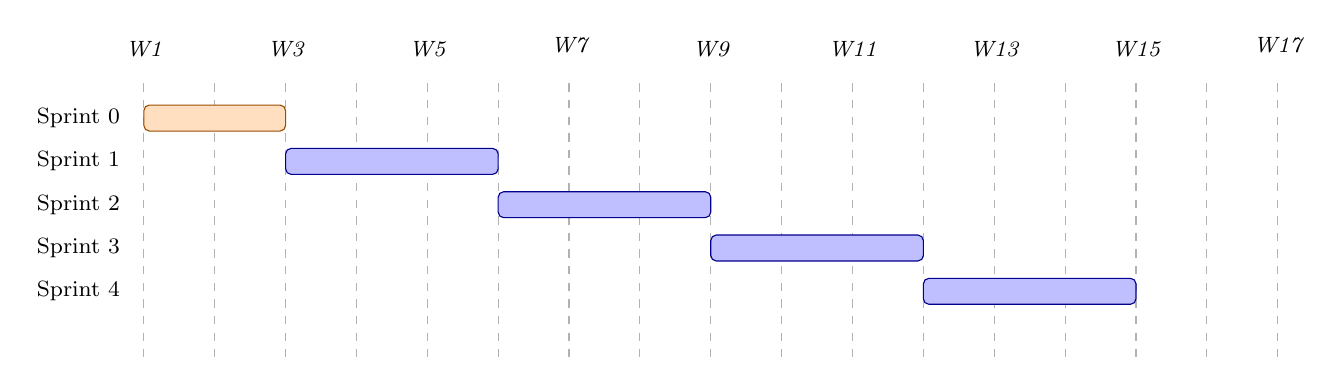
\begin{tikzpicture}[x=0.9cm, y=0.55cm,
  bar/.style={draw=blue!55!black, fill=blue!25, rounded corners=2pt},
  bar0/.style={draw=orange!60!black, fill=orange!25, rounded corners=2pt},
  lbl/.style={font=\footnotesize, anchor=east},
  wk/.style={font=\footnotesize\itshape, anchor=south},
  axis/.style={gray!60}
]
%% Horizontal axis: 16 weeks
\foreach \x in {0,...,16} {
  \draw[axis, dashed] (\x,-0.3) -- (\x,-6.7);
}
\foreach \x/\w in {0/W1, 2/W3, 4/W5, 6/W7, 8/W9, 10/W11, 12/W13, 14/W15, 16/W17} {
  \node[wk] at (\x,0.1) {\w};
}

%% Sprint bars (start, end, y, style, label)
\draw[bar0] (0,-0.8)   rectangle (2,-1.4);   \node[lbl] at (-0.2,-1.1) {Sprint 0};
\draw[bar]  (2,-1.8)   rectangle (5,-2.4);   \node[lbl] at (-0.2,-2.1) {Sprint 1};
\draw[bar]  (5,-2.8)   rectangle (8,-3.4);   \node[lbl] at (-0.2,-3.1) {Sprint 2};
\draw[bar]  (8,-3.8)   rectangle (11,-4.4);  \node[lbl] at (-0.2,-4.1) {Sprint 3};
\draw[bar]  (11,-4.8)  rectangle (14,-5.4);  \node[lbl] at (-0.2,-5.1) {Sprint 4};
\end{tikzpicture}%
}
\caption{Gantt chart of the project sprints}
\label{fig:gantt}
\end{figure}

For clarity, the concrete work completed in each sprint is summarized below:
\begin{itemize}
  \item \textbf{Sprint 0}: Defined actors and use cases, prepared the initial product backlog,
    validated the target architecture, and set up the development environment.
  \item \textbf{Sprint 1}: Implemented authentication and onboarding flows, integrated Stripe
    subscriptions, added AR-API background processing with Celery tasks, and delivered the
    Authentic Rights Portal front-end with a billing and moderation admin workspace.
  \item \textbf{Sprint 2}: Delivered OpenSearch ingestion, BM25 keyword search, facet-based
    filtering (Part A), then semantic embeddings, kNN retrieval, parallel hybrid search, and
    position-aware rank fusion (Part B); also delivered the Video Search Portal front-end and
    playlist management views.
  \item \textbf{Sprint 3}: Built the Agentic Helper RAG foundation with Qdrant retrieval,
    routing/classification, and conversation memory (Phase A), then upgraded to the v2
    deterministic orchestrator, Agentic RAG pipeline, and the Whisper voice transcription
    endpoint (Phase B); also delivered portal-side voice input, the shared ChatbotWidget, and
    AI-backed admin tools (conversation supervision, chatbot tester, FAQ manager).
  \item \textbf{Sprint 4}: Implemented recommendation event tracking, user-interest profiling,
    candidate blending, trending integration, and anti-repetition ranking.
\end{itemize}

\section*{Conclusion}
\addcontentsline{toc}{section}{Conclusion}

This chapter presented BVIRAL as host organization, the specific problems addressed by the
project, the comparative position of the platform against market solutions, and the Scrum-based
sprint plan that drove development. The next chapter enters Sprint 0 and specifies the detailed
requirements, actors, product backlog, work tools, and general architecture.
